% (The MIT License)
%
% Copyright (c) 2023-2024 Yegor Bugayenko
%
% Permission is hereby granted, free of charge, to any person obtaining a copy
% of this software and associated documentation files (the 'Software'), to deal
% in the Software without restriction, including without limitation the rights
% to use, copy, modify, merge, publish, distribute, sublicense, and/or sell
% copies of the Software, and to permit persons to whom the Software is
% furnished to do so, subject to the following conditions:
%
% The above copyright notice and this permission notice shall be included in all
% copies or substantial portions of the Software.
%
% THE SOFTWARE IS PROVIDED 'AS IS', WITHOUT WARRANTY OF ANY KIND, EXPRESS OR
% IMPLIED, INCLUDING BUT NOT LIMITED TO THE WARRANTIES OF MERCHANTABILITY,
% FITNESS FOR A PARTICULAR PURPOSE AND NONINFRINGEMENT. IN NO EVENT SHALL THE
% AUTHORS OR COPYRIGHT HOLDERS BE LIABLE FOR ANY CLAIM, DAMAGES OR OTHER
% LIABILITY, WHETHER IN AN ACTION OF CONTRACT, TORT OR OTHERWISE, ARISING FROM,
% OUT OF OR IN CONNECTION WITH THE SOFTWARE OR THE USE OR OTHER DEALINGS IN THE
% SOFTWARE.

\documentclass{article}
\usepackage{../lecture-notes/notes}
\usepackage{amsmath}
\usepackage{relsize}
\newcommand*\thetitle{Object Dimensions}
\begin{document}

\plush{\lnTitlePage{10}{24}{jdEFoz-OQ44}}

\plush{
\pptBanner{Object Metrics}
\begin{itemize}
  \setlength\itemsep{0em}
  \item Number of attributes, methods, constructors, destructors
  \item Number of static attributes, methods
  \item Number of types/interfaces
  \item Number of parent and child classes
  \item Number of annotations
  \item Number of static blocks
  \item Number of nested classes
  \item Number of type parameters (generics)
\end{itemize}
}

\lnQuote
  [Fernando Brito e Abreu]
  {fernando-brito-e-abreu}
  {\textbf{Metrics for Object-Oriented Design (MOOD)}: Being able to predict some software quality characteristics based on the design, is one of our great motivations. This ability will allow the designing process to be guided, for instance, by means of \ul{heuristics}.}
  {brito1994object}

\pptBanner{Method Hiding Factor (MHF)}
\begin{multicols}{2}
{\small\begin{ffcode}
class Book {
  public String title() {
    return this.read() + ".";
  }
  private String read() {
    // read from database
  }
}
\end{ffcode}
}
\par\columnbreak\par
\(\texttt{MHF}_\texttt{Book} = 1/2\)\par
``MHF is defined as the ratio of the sum of the \ul{invisibilities} of all methods
defined in all classes to the total number of methods defined in the system
under consideration.''
\end{multicols}
\plush{}

\pptBanner{Attribute Hiding Factor (AHF)}
\begin{multicols}{2}
{\small\begin{ffcode}
class Book {
  public int id;
  private File path;
  public String title() {
    var txt = Files.read(path);
    // 1. Find title by 'id'
    // 2. Return it
  }
}

var b = new Book();
b.id = 42;
var t = b.title();
\end{ffcode}
}
\par\columnbreak\par
\(\texttt{AHF}_\texttt{Book} = 1/2\)\par
``AHF is defined as the ratio of the sum of the \ul{invisibilities} of all attributes
defined in all classes to the total number of attributes defined in the system
under consideration.''
\end{multicols}
\plush{}

\pptBanner{Method Inheritance Factor (MIF)}
\begin{multicols}{2}
{\small\begin{ffcode}
class Book extends Material {
  @Override
  public String content() {
    return "Hello, world!";
  }
  public String title() {
    return "David West";
  }
}
\end{ffcode}
}
\par\columnbreak\par
\(\texttt{MIF}_\texttt{Book} = 1/2\)\par
``MIF is defined as the ratio of the sum of the \ul{inherited} methods in all classes of
the system under consideration to the total number of available methods
(locally defined plus inherited) for all classes.''
\end{multicols}
\plush{}

\pptBanner{Attribute Inheritance Factor (AIF)}
\begin{multicols}{2}
{\small\begin{ffcode}
class Material {
  protected String content;
}

class Book extends Material {
  private String title;
}
\end{ffcode}
}
\par\columnbreak\par
\(\texttt{AIF}_\texttt{Book} = 1/2\)\par
``AIF is defined as the ratio of the sum of \ul{inherited} attributes in all classes of
the system under consideration to the total number of available attributes
(locally defined plus inherited) for all classes.''
\end{multicols}
\plush{}

\pptBanner{Polymorphism Factor (PF)}
\begin{multicols}{2}
{\small\begin{ffcode}
class Material {
  public String content() {
    return "Hello, world!";
  }
}

class Book extends Material {
  public String title() {
    return "David";
  }
}
\end{ffcode}
}
\par\columnbreak\par
\(\texttt{PF}_\texttt{Book} = 0/1\)\par
``PF is the number of methods that \ul{redefine} inherited methods, divided by the
maximum number of possible distinct polymorphic situations.''
\end{multicols}
\plush{}

\lnQuote
  [Chris F. Kemerer]
  {chris-kemerer}
  {The inheritance hierarchy, a directed acyclic graph will be described as a tree structure with classes as nodes, leaves and a root. In any design application, there can be many possible \ul{hierarchies of classes}. Design choices on the hierarchy employed to represent the application are essentially choices about restricting or expanding the scope of properties of the objects in the application.}
  {chidamber1994metrics}

\pptBanner{Weighted Methods per Class (WMC)}
\begin{multicols}{2}
Consider a class \(C_i\), with methods \(M_1, \dots, M_n\). Let \(c_1, \dots, c_n\) be
the complexity of the methods. Then:
\begin{equation*}
\text{WMC} = \sum_{i=1}^{n} c_i
\end{equation*}
If all method complexities are considered to be unity, then \(\text{WMC} = n\),
the number of methods.
\par\columnbreak\par
``It can be argued that developers approach the task of writing a method as they would
a traditional program, and therefore some traditional static complexity metric,
such as McCabe's Cyclomatic number, may be appropriate.''
\lnSource{chidamber1994metrics}
\end{multicols}
\plush{}

\pptBanner{Depth of Inheritance Tree (DIT)}
\begin{multicols}{2}
{\small\begin{ffcode}
class Material {
  public String content() {
    return "Hello, world!";
  }
}

class Book (*@\textcolor{orange}{extends Material}@*) {
  public String title() {
    return "David";
  }
}
\end{ffcode}
}
\par\columnbreak\par
\(\texttt{DIT}_\texttt{Material} = 0\)\par
\(\texttt{DIT}_\texttt{Book} = 1\)\par
``DIT is a measure of how many \ul{ancestor} classes can potentially affect this class.''
\end{multicols}
\plush{}

\pptBanner{Number of Children (NOC)}
\begin{multicols}{2}
{\small\begin{ffcode}
class Material {
  public String content() {
    return "Hello, world!";
  }
}

class Book (*@\textcolor{orange}{extends Material}@*) {
  public String title() {
    return "David";
  }
}
\end{ffcode}
}
\par\columnbreak\par
\(\texttt{NOC}_\texttt{Material} = 1\)\par
\(\texttt{NOC}_\texttt{Book} = 0\)\par
``NOC is a measure of how many \ul{sub-classes} are going to inherit the methods of the parent class.''
\end{multicols}
\plush{}

\pptBanner{Response For a Class (RFC)}
\begin{multicols}{2}
{\small\begin{ffcode}
class Trim
  String value()

class Book
  public String (*@\textcolor{orange}{title}@*)()
    return new Trim(
      this.(*@\textcolor{orange}{read}@*)()
    ).(*@\textcolor{orange}{value}@*)();
  private String (*@\textcolor{orange}{read}@*)()
    // read from the DB
\end{ffcode}
}
\par\columnbreak\par
\(\texttt{RFC}_\texttt{Book} = 3\)\par
``RFC is the count of the set of \ul{all methods} that can be invoked in response to a message to an object of the class or by some method in the class.''
\end{multicols}
\plush{}

\lnPitch{
  \begin{multicols}{2}
  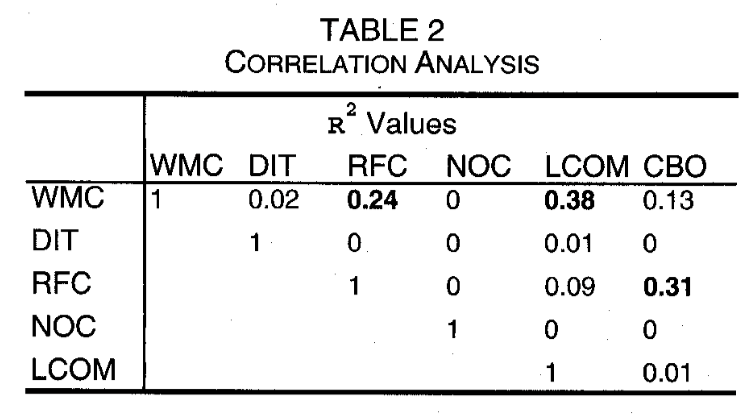
\includegraphics[width=\linewidth]{correlation.png}
  \par\columnbreak\par
  Table shows very clearly that linear Pearson's correlations
  between the studied OO metrics are, in general, very weak.
  We conclude that these metrics are mostly statistically
  independent and, therefore, do not capture a great deal
  of redundant information.
  \lnSource{basili1996validation}
  \end{multicols}}

\lnQuote
  {../10-object-dimensions/book}
  {A small number of classes may be responsible for a large number of the methods that executed in an application, and that if testing effort were concentrated on these outlier classes, a bulk of the dynamic behavior of the object oriented systems can be checked for customer acceptance.}
  {chidamber1994metrics}

\lnQuote
  [Mark Lorenz]
  {mark-lorenz}
  {Number of Messages (NOM) measures the number of messages sent in a method, segregated by type of message.}
  {lorenz1994object}

\pptBanner{Number of Messages (NOM)}
\begin{multicols}{2}
{\small\begin{ffcode}
class Trim
  String value()

class Book
  public String title()
    return (*@\textcolor{orange}{new}@*) Trim(
      this(*@\textcolor{orange}{.read}@*)()
    )(*@\textcolor{orange}{.value}@*)();
  private String read()
    // read from the DB
\end{ffcode}
}
\par\columnbreak\par
\(\texttt{NOM}_\texttt{title} = 3\)\par
``Number of Messages (NOM) measures the number of messages sent in a method, segregated by type of message.''
\end{multicols}
\plush{}

\end{document}
